\documentclass[10pt,twocolumn,letterpaper]{article}

\usepackage{iccv}
\usepackage{times}
\usepackage{epsfig}
\usepackage{graphicx}
\usepackage{amsmath}
\usepackage{amssymb}
\usepackage{comment}
\usepackage{algorithm2e}
\usepackage{color}

%\renewcommand{\baselinestretch}{0.96}
\renewcommand{\floatsep}{6pt}
\renewcommand{\dblfloatsep}{3pt}
\renewcommand{\textfloatsep}{6pt}
\renewcommand{\dbltextfloatsep}{6pt}
\addtolength{\topsep}{-3pt}
\addtolength{\partopsep}{-3pt}
\addtolength{\itemsep}{-3pt}

% Include other packages here, before hyperref.

% If you comment hyperref and then uncomment it, you should delete
% egpaper.aux before re-running latex.  (Or just hit 'q' on the first latex
% run, let it finish, and you should be clear).
\usepackage[breaklinks=true,bookmarks=false]{hyperref}

\iccvfinalcopy % *** Uncomment this line for the final submission

\def\iccvPaperID{****} % *** Enter the ICCV Paper ID here
\def\httilde{\mbox{\tt\raisebox{-.5ex}{\symbol{126}}}}

% Pages are numbered in submission mode, and unnumbered in camera-ready
%\ificcvfinal\pagestyle{empty}\fi
\setcounter{page}{4321}
\begin{document}

%%%%%%%%% TITLE
\title{Look and Think Twice: Capturing Top-Down Visual Attention with Feedback Convolutional Neural Networks\thanks{This work is conducted during Chunshui Cao's and Xianming Liu's internship at Institute of Deep Learning, Baidu Research }}


\author{Chunshui Cao$^\dag$ \;\; Xianming Liu$^\ddag$ \;\; Yi Yang$^\S$ \;\; Yinan Yu$^\natural$ \;\; \\
Deva Ramanan$^\sharp$ \;\; Tieniu Tan$^\dag$ \;\; Thomas S. Huang$^\ddag$ \\
$^\dag$Institute of Automation, Chinese Academy of Science\\
$^\ddag$Beckman Institute, University of Illinois at Urbana-Champaign\\
$^\S$Baidu Research \quad $^\natural$Horizontal Robotics\\
$^\sharp$Carnegie Mellon University \\
{\tt \small \{***\}@ia.ac.cn \;\; \{xliu102,t-huang1\}@illinois.edu \;\; yangyi05@baidu.com \;\;}\\
{\tt \small ***@***.com \;\; deva@cs.cmu.edu }
}

\maketitle
%\thispagestyle{empty}


%%%%%%%%% ABSTRACT
\begin{abstract}
While feedforward deep convolutional neural networks (CNNs) have been a great success in computer vision, it is important to note that the human visual cortex generally contains more feedback than feedforward connections.
In this paper, we will briefly introduce the background of feedbacks in the human visual cortex, which motivates us to develop a computational feedback mechanism in deep neural networks.
In addition to the feedforward inference in traditional neural networks, a feedback loop is introduced to infer the activation status of hidden layer neurons according to the ``goal'' of the network, e.g., high-level semantic labels.
We analogize this mechanism as ``\textbf{Look and Think Twice}.''
The feedback networks help better visualize and understand how deep neural networks work, and capture visual attention on expected objects, even in images with cluttered background and multiple objects.
Experiments on ImageNet dataset demonstrate its effectiveness in solving tasks such as classification and object localization.
\end{abstract}

%%%%%%%%% BODY TEXT
\section{Introduction}

% Start with a little story
\begin{center}
  \fbox{
    \parbox{0.85\linewidth}{
    \noindent
    \emph{``What did you see in this image?''\\
      ``Panda, Tiger, Elephant, Lions.''\\
      ``Have you seen the Gorilla?''\\
      ``Oh! I even didn't notice there is a Gorilla !''}
    }
  }
\end{center}

\setlength{\tabcolsep}{2pt}
\begin{figure}[htb]
\begin{center}
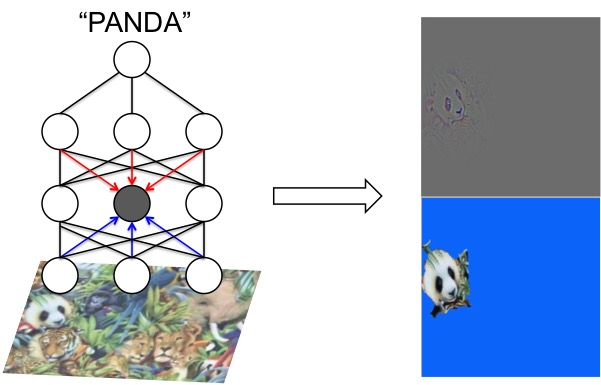
\includegraphics[width=0.9\columnwidth]{figs/splash0/splash}
\caption{Feedback Convolutional Net model for capturing visual attention by inferring the status of hidden neuron activations. It is designed to utilize both bottom-up image inputs and top-down semantic labels to infer the hidden neuron activations. Salient areas captured by feedback often correspond to related ``target'' objects, even in images with cluttered background and multiple objects.}
\label{fig:splash0}
\end{center}
\end{figure}

Visual attention typically is dominated by \emph{``goals''} from our mind easily in a top-down manner, especially in the case of object detection. Cognitive science explains this in the ``Biased Competition Theory''~\cite{beck2009top,desimone1998visual,desimone1995neural}, that human visual cortex is enhanced by top-down stimuli and non-relevant neurons will be suppressed in feedback loops when searching for objects. By ``\emph{looking and thinking twice}'', both human recognition and detection performances increase significantly, especially in images with cluttered background~\cite{Cichy2014Resolving}. This leads to the selectivity in neuron activations~\cite{Kruger2013Deep}, which reduces the chance of recognition being interfered with either noises or distractive patterns.

Inspired by above evidences, we present a novel \emph{Feedback Convolutional Neural Network} architecture in this paper. It achieves this selectivity by jointly reasoning outputs of class nodes and activations of hidden layer neurons during the feedback loop. As shown in Figure~\ref{fig:splash0}, during the feedforward stage, the proposed networks perform inference from input images in a bottom-up manner as traditional Convolutional Networks; while in feedback loops, it sets up high-level semantic labels, (\emph{e.g.}, outputs of class nodes) as the ``goal'' in visual search to infer the activation status of hidden layer neurons. We show that the network is powerful enough to apply for class model visualization~\cite{simonyan2013deep, zeiler2014visualizing}, object localization~\cite{simonyan2013deep} and image classification~\cite{Krizhevsky2012ImageNet}.

\setlength{\tabcolsep}{0.5pt}
\begin{figure*}[htb]
\begin{center}
\begin{tabular}{ccccccc}
%\rotatebox{90}{\hspace{5mm}Sequential} &
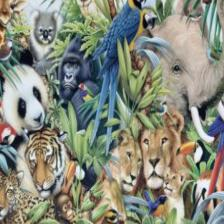
\includegraphics[width=0.14\linewidth]{figs/splash/original} &

\includegraphics[width=0.14\linewidth]{figs/splash/panda} &

\includegraphics[width=0.14\linewidth]{figs/splash/tiger} &

\includegraphics[width=0.14\linewidth]{figs/splash/gorilla} &

\includegraphics[width=0.14\linewidth]{figs/splash/lion} &

\includegraphics[width=0.14\linewidth]{figs/splash/elephant} &
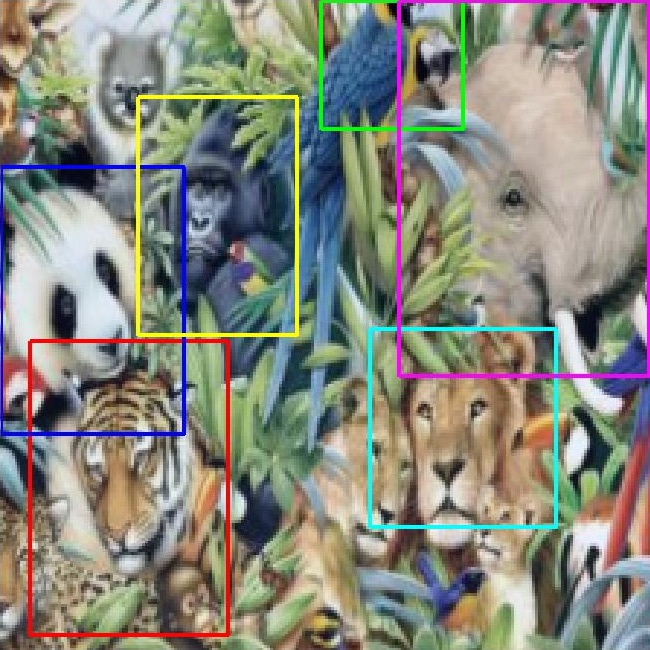
\includegraphics[width=0.14\linewidth]{figs/splash/localization}\\
{\small (a) Input Image} &
{\small (b) Panda} &
{\small (c) Tiger} &
{\small (d) Gorilla} &
{\small (e) Lion} &
{\small (f) Elephant} &
{\small (g) Localization}
\end{tabular}
\caption{We illustrate the localization power of the feedback net on a multi-object image with cluttered background. (a) shows the original input image which both VggNet~\cite{Simonyan2014Very} and GoogleNet~\cite{Szegedy2014Going} recognize as "comic book". (b) - (f) illustrate our feedback model on understanding the image given different class labels as a prior. We visualize the gradient of each class node with respect to image after the feedback net finish its inference. (g) shows the final localizations for different objects based on the gradients. Better viewed in color.}
\label{fig:splah}
\end{center}
\end{figure*}

\textbf{Optimization in a Feedback Loop}:
% Explain from the machine learning perspective
From a machine learning perspective, the proposed feedback networks \emph{add extra flexibility to Convolutional Networks, to help in capturing visual attention and improving feature detection}. Convolutional Neural Networks~\cite{lecun1998gradient, Krizhevsky2012ImageNet, Simonyan2014Very} have achieved great success in both machine learning and computer vision in recent years. Benefiting from large-scale training data, (\emph{e.g.,} ImageNet~\cite{deng2009imagenet}), CNNs are capable of learning filters and image compositions at the same time. Various approaches have been adopted to further increase generalization ability of CNNs, by either adding regularization in training~\cite{he2015delving,ioffe2015batch}, or going deeper~\cite{Simonyan2014Very, Szegedy2014Going}. Inspired by Deformable Part-Based Models (DPMs)~\cite{Felzenszwalb2010Object} that characterize middle level part locations as latent variables and search for them during object detection, we utilize a simple yet efficient method to optimize image compositions and assign neuron activations given ``goals'' in visual search. The algorithm maximizes the posterior response of network given target high-level semantic concepts, in a top-down manner. Compared with traditional bottom-up strategies~\cite{he2015delving, ioffe2015batch}, which aim to regularize the network training, the proposed feedback framework adds flexibilities to the model inference from high-level concepts down to the receptive field.

Figure~\ref{fig:splah} shows an example on how this flexibility is reflected in detection and localization. Instead of recognizing the input image as a ``comic book'', the proposed feedback network is capable to localize each component of the ``comic book'' via salience maps. The example shown in Figure~\ref{fig:splash0} illustrates its working mechanism: given a high-level semantic stimulus ``PANDA'', only the neurons in hidden layers related with the concept ``PANDA'' will be activated by iterative optimization in a feedback loop. As a result, only salient regions related with the concept ``PANDA'' are captured in visualizations.
As suggested by those results, the feedback networks achieve certain level of selectivity and provide non-relevant suppression during the top-down inference, allowing the model to focus on the most salient image regions that improve the class confidence.

% Unify the network: recognition and detection in a single network.
% Simultaneously answer the question of "what" and "where"
\textbf{Weakly Supervised Object Localization}:
Given gradient visualizations in Figure~\ref{fig:splah}, we further develop an algorithm for weakly supervised object localization. Instead of using large amount of supervision (\emph{e.g.}, bounding box positions) in traditional methods such as R-CNN~\cite{girshick2014rich} or using regression model~\cite{erhan2014scalable, Simonyan2014Very}, we don't require any localization information in the training stage. Instead, we adopt \emph{a unified network performing both recognition and localization tasks}, to answer questions of ``what'' and ``where'' simultaneously, which are the two most important tasks in computer vision. Experimental results suggest that our weakly supervised algorithm using feedback network could achieve similar performance on ImageNet object localization task as GoogLeNet~\cite{Szegedy2014Going} and VGG~\cite{Simonyan2014Very}.

% Newly added to say something about the classification task
\textbf{Image Classification Revisited}:
We mimic the human visual recognition process that human may focus to recognize objects in a complicated image after a first time glimpse as the procedure ``Look and Think Twice'' for image classification. We utilize the weakly supervised object localization during the ``first glimpse'' to make guesses of ROIs, then make the network refocused on those ROIs and give final classifications list. Experimental results on ImageNet 2014 classification validation dataset suggest that this approach is efficient to eliminate irrelevant clutters and improve classification accuracy especially on small objects.


%\setlength{\tabcolsep}{2pt}
%\begin{figure*}
%\begin{center}
%\begin{tabular}{ccccccccc}
%\rotatebox{90}{\hspace{5mm}Oxford} &
%
\includegraphics[width=0.11\linewidth]{figs/visual_compare/gradient/oxford/panda} &
%
\includegraphics[width=0.11\linewidth]{figs/visual_compare/saliency/oxford/panda} &
%
\includegraphics[width=0.11\linewidth]{figs/visual_compare/gradient/oxford/tiger} &
%
\includegraphics[width=0.11\linewidth]{figs/visual_compare/saliency/oxford/tiger} &
%
\includegraphics[width=0.11\linewidth]{figs/visual_compare/gradient/oxford/gorilla} &
%
\includegraphics[width=0.11\linewidth]{figs/visual_compare/saliency/oxford/gorilla} &
%
\includegraphics[width=0.11\linewidth]{figs/visual_compare/gradient/oxford/lion} &
%
\includegraphics[width=0.11\linewidth]{figs/visual_compare/saliency/oxford/lion} \\
%\rotatebox{90}{\hspace{5mm}Deconv} &
%
\includegraphics[width=0.11\linewidth]{figs/visual_compare/gradient/deconv/panda} &
%
\includegraphics[width=0.11\linewidth]{figs/visual_compare/saliency/deconv/panda} &
%
\includegraphics[width=0.11\linewidth]{figs/visual_compare/gradient/deconv/tiger} &
%
\includegraphics[width=0.11\linewidth]{figs/visual_compare/saliency/deconv/tiger} &
%
\includegraphics[width=0.11\linewidth]{figs/visual_compare/gradient/deconv/gorilla} &
%
\includegraphics[width=0.11\linewidth]{figs/visual_compare/saliency/deconv/gorilla} &
%
\includegraphics[width=0.11\linewidth]{figs/visual_compare/gradient/deconv/lion} &
%
\includegraphics[width=0.11\linewidth]{figs/visual_compare/saliency/deconv/lion} \\
%\rotatebox{90}{\hspace{5mm}Our} &
%
\includegraphics[width=0.11\linewidth]{figs/visual_compare/gradient/feedback/panda} &
%
\includegraphics[width=0.11\linewidth]{figs/visual_compare/saliency/feedback/panda} &
%
\includegraphics[width=0.11\linewidth]{figs/visual_compare/gradient/feedback/tiger} &
%
\includegraphics[width=0.11\linewidth]{figs/visual_compare/saliency/feedback/tiger} &
%
\includegraphics[width=0.11\linewidth]{figs/visual_compare/gradient/feedback/gorilla} &
%
\includegraphics[width=0.11\linewidth]{figs/visual_compare/saliency/feedback/gorilla} &
%
\includegraphics[width=0.11\linewidth]{figs/visual_compare/gradient/feedback/lion} &
%
\includegraphics[width=0.11\linewidth]{figs/visual_compare/saliency/feedback/lion} \\
%&
%\multicolumn{2}{c}{{\small (a) Panda}} &
%\multicolumn{2}{c}{{\small (b) Tiger}} &
%\multicolumn{2}{c}{{\small (c) Gorilla}} &
%\multicolumn{2}{c}{{\small (d) Lion}} \\
%\end{tabular}
%% \vspace{-10pt}
%\caption{We demonstrate the effectiveness of our method by comparing the class model visualization results against Oxford~\cite{simonyan2013deep} and Deconv~\cite{zeiler2014visualizing}. The input image is the same as Figure 1 (a). We show both the visualization results as well as the saliency map. While both Oxford and Deconv have the same input: the image and an object class label (i.e. tiger, panda, etc.), the gradients computed are often salient on one particular object (i.e. elephant). Our feedback framework allows for the model to focus on the most important image area that improves the class confidence.}
%\label{fig:visual_compare}
%% \vspace{-30pt}
%\end{center}
%\end{figure*}

\section{Related Work}
\label{sec:related_work}

% Organization: 1) feedforward cnn 2) feedback network: RBM, Deconvolution, RNN. 3) visualization and attention 4) localization and detection
\subsection{Feedforward and Feedback Mechanism}
Deep Neural Network takes a \emph{feedforward-Back Error Propagation} strategy to learn features and classifiers simultaneously, from large scale of training samples~\cite{Krizhevsky2012ImageNet,Simonyan2014Very,lin2013network,salakhutdinov2009deep,bengio2013representation}. Various approaches have been proposed to further improve the discriminative ability of deep neural network, either by 1) adding regularization to improve the robustness of learnt model and get rid of overfitting, such as Dropout~\cite{srivastava2014dropout}, PReLU~\cite{he2015delving}, Batch Normalization~\cite{ioffe2015batch}; or 2) making the network deeper~\cite{Szegedy2014Going,Simonyan2014Very}.

Despite great successes achieved by applying Feedforward Networks to image recognition and detection, evidences accumulate from cognitive studies and point to the feedback mechanism that may dominant human perception processes~\cite{Cichy2014Resolving,Rust:2010if,Kruger2013Deep,lee2003hierarchical}. Recently, tentative efforts have been made to involve feedback strategy into Deep Neural Networks. Deep Boltzmman Machines
(DBM)~\cite{salakhutdinov2009deep,sohn2013learning} and Deconvolutional Nerual Networks~\cite{Zeiler:2011hy} try to formulate the feedback as a reconstruction process within the training stage. Meanwhile, Recurrent Neural Networks (RNN) and Long Short Term Memory (LSTM)~\cite{hochreiter1997long} are utilized to capture the attention drifting in a dynamic environment and learn the feedback mechanisms via reinforcement learning~\cite{Stollenga:2014tl,Mnih:2014ti}. DRAW from Google
DeepMind~\cite{gregor2015draw} combine above two into a generative model, to synthesize the image generation process.

As in \emph{Biased Competition Theory}~\cite{beck2009top,desimone1995neural}, feedback, which passes the high-level semantic information down to the low-level perception, controls the selectivity of neuron activations in an extra loop in addition to the feedforward process. This results in the ``Top-Down'' attention in human cognition. Hierarchical probabilistic computational models~\cite{lee2003hierarchical} are proposed to characterize feedback stimuli in a top-down manner, which are further incorporated into deep neural networks, for example, modeling feedback as latent variables in DBM~\cite{wang2014attentional}, or using selectivity to resolve fine-grained classification~\cite{Mnih:2014ti}, \emph{et al.}. However, generative models used in~\cite{Mnih:2014ti,wang2014attentional} are limited by low computational efficiency and capacity, and are hardly used in large scale datasets.

\subsection{Visualization, Detection, and Localization}

Feedback is often related with visualization of CNN and object localization since both of them aim to project the high-level semantic information back to image representations. To visualize neuron responses and class models, various approaches are proposed either using deconvolution~\cite{zeiler2014visualizing} or optimization based on gradients~\cite{simonyan2013deep, le2013building}. As demonstrated in \cite{simonyan2013deep}, visualization of Convolutional Neural Network shows semantically meaningful salient object regions and helps understand working mechanism of CNNs.

Object detection and localization are more about feedback, by treating detection / localization as a searching process with clear ``goals.'' To localize and detect objects in images, typical approaches use supervised training, which relies on large amount of supervision, \emph{e.g.}, ground-truth bounding boxes, or manually labeled segmentation in training samples~\cite{erhan2014scalable}. To behave ``searching'', sliding window is used~\cite{erhan2014scalable}, or instead region proposals detected by image segmentations~\cite{uijlings2013selective} in R-CNN~\cite{girshick2014rich}. However, both of these approaches are computational intensive and naturally bottom-up: selecting candidate regions, performing feedforward classification and making decisions.

Inspired by visualizations of CNNs~\cite{zeiler2014visualizing,simonyan2013deep}, a more feasible and cognitive manner for detection / localization could be derived by utilizing the saliency maps generated in feedback visualizations. Moreover, an ideal approach should unify the recognition and detection in a single feedforward-feedback network architecture. However, if possible, the challenge lies on how to obtain semantically meaningful salience maps with high quality for each concept. That's the ultimate goal of our work presented in this paper.

\section{Model}
\label{sec:model}

\setlength{\tabcolsep}{2pt}
\begin{figure*}
\begin{center}
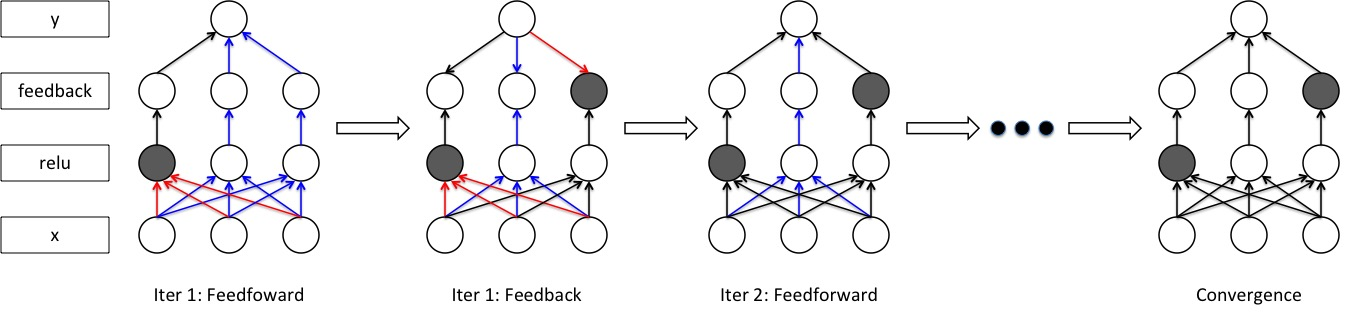
\includegraphics[width=\linewidth]{figs/model/model}
% \vspace{-10pt}
\caption{Illustration of our feedback model and its inference process. At the first iteration, the model performs as a feedforward neural net. Then, the neurons in the feedback hidden layers update their activation status to maximize the confidence output of the target top neuron. This process continues until convergence. (We show only one layer here, but feedback layers can be tacked in the deep ConvNet.)}
\label{fig:model}
% \vspace{-30pt}
\end{center}
\end{figure*}


\subsection{Re-interpreting ReLU and Max-Pooling}
The most recent state-of-the-art deep CNNs~\cite{Simonyan2014Very} consist of many stacked feedforward layers, including convolutional, rectified linear units (ReLU) and max-pooling layers. For each layer, the input $\mathbf{x}$ can be an image or the output of a previous layer, consisting of $C$ input channels of width $M$ and height $N$: $\mathbf{x} \in \mathcal{R}^{M \times N \times C}$. The output $\mathbf{y}$ consists of a set of $C'$ output channels of width $M'$ and height $N'$: $\mathbf{y} \in \mathcal{R}^{M' \times N' \times C'}$.

\emph{Convolutional Layer:}
The convolution layer is used to extract different features of the input. The convolutional layer is parameterized by $C'$ filters with every filter $\mathbf{k} \in \mathcal{R}^{K \times K \times C}$.
\begin{equation}
\mathbf{y}_{c'} = \sum_{c=1}^C \mathbf{k}_{c'c} * \mathbf{x}_c,\ \forall c'
\end{equation}

\emph{ReLU Layer:}
The ReLU layer is used to increase the nonlinear properties of the decision function and of the overall network without affecting the receptive fields of the convoluional layer.
\begin{equation}
\mathbf{y} = \max (\mathbf{0}, \mathbf{x})
\label{eq:relu}
\end{equation}

\emph{Max-Pooling Layer:}
The max-pooling layer is used to reduce the dimensionality of the output and variance in deformable objects to ensure that the same result will be obtained even when image features have small translations. The max-pooling operation is applied for every pixel $(i,j)$ around its small neighborhood $\mathcal{N}$.
\begin{equation}
y_{i,j,c} = \max_{u,v \in \mathcal{N}} x_{i+u, j+v, c},\ \forall i, j, c
\label{eq:max-pool}
\end{equation}


\textbf{Selectivity in Feedward Network:}
To better understand how selectivity works in neural networks and how to formulate the feedback, we re-interpret behaviors of ReLU and Max-Pooling layers as a set of binary activation variables $\mathbf{z} \in \{0,1\}$ instead of the $\max()$ operation in Equation~\ref{eq:relu}~and~\ref{eq:max-pool}. Thus, behaviors of ReLU and Max-Pooling could be formulated as $\mathbf{y} = \mathbf{z} \circ \mathbf{x}$, where $\circ$ is the element wise product (Hadamard product); and $\mathbf{y} = \mathbf{z} * \mathbf{x}$, where $*$ is the convolution operator and $\mathbf{z}$ is a set of convolutional filters except that they are location variant.

Be interpreting ReLU and Max-Pooling layers as ``gates'' controlled by input $x$, the network selects information during feedforward phases in a \emph{bottom-up} manner, and eliminates signals with minor contributions in making decisions. However, the activated neurons could be either helpful or harmful for classification, and involve too many noises, for instance, cluttered backgrounds in complex scenes.

\subsection{Introducing the Feedback Layer}
Since the model opens all gates and allow maximal information getting through to ensure the generalization, to increase the discriminability within feature level, it is feasible to turn off those gates that provide irrelevant information when targeting at particular semantic labels. This strategy is explained as selectivity in biased competition theory~\cite{desimone1995neural} and is critical to realize the top-down attention.

More technically, to increase the model flexibility to images and prior knowledges, we introduce an extra layer to the existing convolutional neural network. We call it the \emph{feedback layer}. The feedback layer contains another set of binary neuron activation variables $\mathbf{z} \in \{0, 1\}$, in addition to ReLU. However, these binary variables are activated by top-down messages from outputs, instead of bottom inputs.
%
The feedback layer is stacked upon each ReLU layer, and they compose a hybrid control unit to active neuron response in both bottom-up and top-down manners:

\begin{description}
  \item[Bottom-Up] Inherent the selectivity from \emph{ReLU layers}, and the dominant features will be passed to upper layers;
  \item[Top-Down] Controlled by \emph{Feedback Layers}, which propagate the high-level semantics and global information back to image representations. Only those gates related with particular target neurons are activated.
\end{description}
Figure.~\ref{fig:model} illustrates a simple architecture of our feedback model with only one ReLU layer and one feedback layer.

\subsection{Updating Hidden Neurons in Feedback Loops}
We formulate the feedback mechanism as an optimization problem, by introducing an addition control gate-variable $\mathbf{z}$. Given an image $I$ and a neural network with learned parameters $w$, we optimize the target neuron output by jointly inference on binary neuron activations $\mathbf{z}$ over all the hidden feedback layers. In particular, if the target neuron is a $k$-th class node in the top layer, we optimize the class score $s_k$ by re-adjusting the neuron activations at every neuron $(i,j)$ of channel $c$, on feedback layer $l$.
\begin{equation}
\begin{aligned}
& \max_\mathbf{z} & & s_k(I, \mathbf{z}) - \lambda ||\mathbf{z}|| \\
& s.t. & & \ z^l_{i,j,c} \in \{0, 1\}, \; \forall\ l, i, j, c
\end{aligned}
\end{equation}
Since the goal of this optimization aims at activating minimal number of neurons yet maximizing the target score, we use $L1$ norm in above target function, as $\|\mathbf{z}\|_1$


This leads to an integer programming problem, which is NP-hard given the current deep net architecture. An approximation could be derived by applying a linear relaxation:
\begin{equation}
\begin{aligned}
& \max_\mathbf{z} & & s_k(I, \mathbf{z}) - \lambda ||\mathbf{z}||_1 \\
& s.t. & & \ 0 \leq z^l_{i,j,c} \leq 1, \; \forall\ l, i, j, c\\
\end{aligned}
\end{equation}

We use the gradient ascent algorithm to update the hidden variables through all layers simultaneously.
\begin{equation}
\begin{aligned}
\mathbf{z}_{t+1} = \mathbf{z}_t + \alpha \cdot (\frac{\partial s_k}{\partial \mathbf{z}} |_{\mathbf{z}_t} - \lambda)
\end{aligned}
\end{equation}
where $\frac{\partial \lambda \|\mathbf{z}\|_1}{\partial z_i} = \lambda$ since we require $0 \leq z^l_{i,j,c} \leq 1$.

The initialization of feedback layer status $z$ is set to be the corresponding ReLU activation after the first feedforward pass and truncate $z$ when the updated values are either larger than 1 or smaller than 0 during inference.

\subsection{Implementation Details}
As for the implementation details, we set the feedback layer on top of each ReLU layer. We intialize all the hidden activations from $\mathbf{z}=\mathbf{1}$, making all feedback ``gates'' opening during the first time feedforward pass. It is suspected that fully connected layers learn embedding spaces rather than particular parts compared to convolutional layers. We update high level feedback layers according to the sign of gradient of each neuron. We set learning rate of hidden activations to 0.1 and update the neurons of all the feedback layers simultaneously. Each iteration performs a feedforward step of the neural net and a backpropagation step to send back gradients. We stop this process in 10 to 50 iterations.

\section{Experimental Results}
\label{sec:experiment}

\setlength{\tabcolsep}{0.5pt}
\begin{figure*}
\begin{center}
\begin{tabular}{ccccccc}
& \multicolumn{3}{c}{\small -------------------- Object 1: dog --------------------} & \multicolumn{3}{c}{\small -------------------- Object 2: cat --------------------} \\
\vspace{-2.5pt}
%
\includegraphics[width=0.14\linewidth,height=0.115\linewidth]{figs/examples/googlenet/oxford/dog-cat1} &
%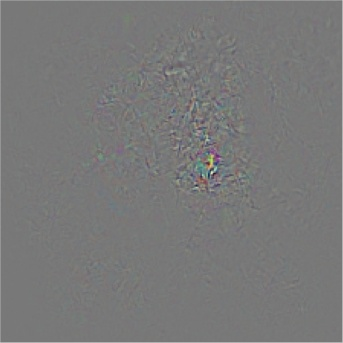
\includegraphics[width=0.14\linewidth,height=0.115\linewidth]{figs/examples/googlenet/oxford/dog-cat1_diff_258} &
%
\includegraphics[width=0.14\linewidth,height=0.115\linewidth]{figs/examples/googlenet/deconv/dog-cat1_diff_258} &
%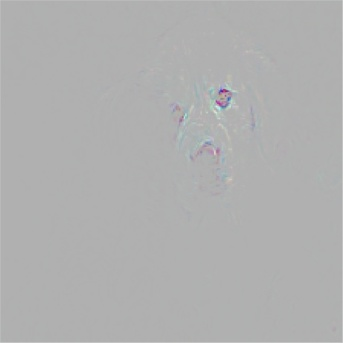
\includegraphics[width=0.14\linewidth,height=0.115\linewidth]{figs/examples/googlenet/soft/dog-cat1_diff_258} &
%
\includegraphics[width=0.14\linewidth,height=0.115\linewidth]{figs/examples/googlenet/oxford/dog-cat1_diff_286} &
%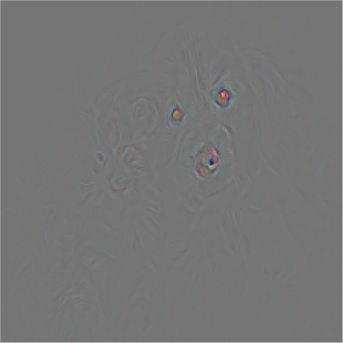
\includegraphics[width=0.14\linewidth,height=0.115\linewidth]{figs/examples/googlenet/deconv/dog-cat1_diff_286} &
%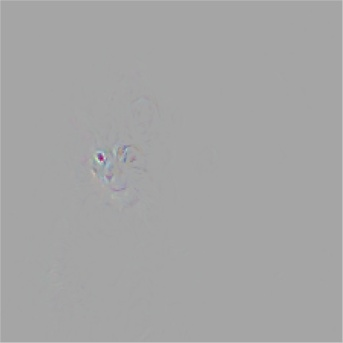
\includegraphics[width=0.14\linewidth,height=0.115\linewidth]{figs/examples/googlenet/soft/dog-cat1_diff_286} \\
%\vspace{-2.5pt}

\includegraphics[width=0.14\linewidth,height=0.115\linewidth]{figs/examples/googlenet/oxford/dog-cat2} &

\includegraphics[width=0.14\linewidth,height=0.115\linewidth]{figs/examples/googlenet/oxford/dog-cat2_diff_163} &

\includegraphics[width=0.14\linewidth,height=0.115\linewidth]{figs/examples/googlenet/deconv/dog-cat2_diff_163} &
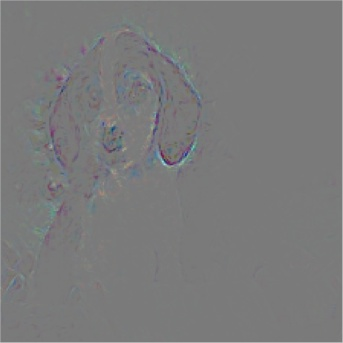
\includegraphics[width=0.14\linewidth,height=0.115\linewidth]{figs/examples/googlenet/soft/dog-cat2_diff_163} &

\includegraphics[width=0.14\linewidth,height=0.115\linewidth]{figs/examples/googlenet/oxford/dog-cat2_diff_286} &
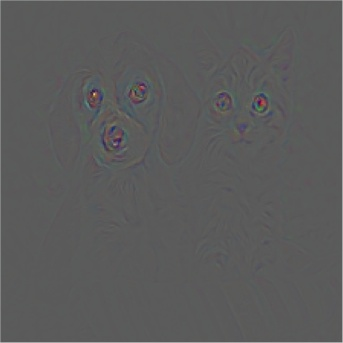
\includegraphics[width=0.14\linewidth,height=0.115\linewidth]{figs/examples/googlenet/deconv/dog-cat2_diff_286} &
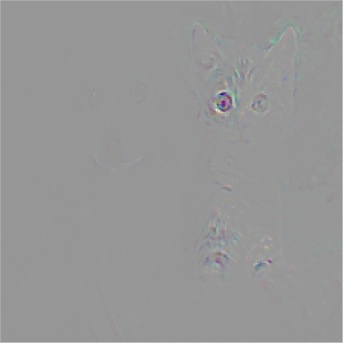
\includegraphics[width=0.14\linewidth,height=0.115\linewidth]{figs/examples/googlenet/soft/dog-cat2_diff_286} \\
\vspace{-2.5pt}
%
\includegraphics[width=0.14\linewidth,height=0.115\linewidth]{figs/examples/googlenet/oxford/dog-cat3} &
%
\includegraphics[width=0.14\linewidth,height=0.115\linewidth]{figs/examples/googlenet/oxford/dog-cat3_diff_188} &
%
\includegraphics[width=0.14\linewidth,height=0.115\linewidth]{figs/examples/googlenet/deconv/dog-cat3_diff_188} &
%\includegraphics[width=0.14\linewidth,height=0.115\linewidth]{figs/examples/googlenet/soft/dog-cat3_diff_188} &
%\includegraphics[width=0.14\linewidth,height=0.115\linewidth]{figs/examples/googlenet/oxford/dog-cat3_diff_286} &
%\includegraphics[width=0.14\linewidth,height=0.115\linewidth]{figs/examples/googlenet/deconv/dog-cat3_diff_286} &
%\includegraphics[width=0.14\linewidth,height=0.115\linewidth]{figs/examples/googlenet/soft/dog-cat3_diff_286} \\
%\vspace{-2.5pt}
\includegraphics[width=0.14\linewidth,height=0.115\linewidth]{figs/examples/googlenet/oxford/dog-cat4} &
\includegraphics[width=0.14\linewidth,height=0.115\linewidth]{figs/examples/googlenet/oxford/dog-cat4_diff_243} &
\includegraphics[width=0.14\linewidth,height=0.115\linewidth]{figs/examples/googlenet/deconv/dog-cat4_diff_243} &
\includegraphics[width=0.14\linewidth,height=0.115\linewidth]{figs/examples/googlenet/soft/dog-cat4_diff_243} &
\includegraphics[width=0.14\linewidth,height=0.115\linewidth]{figs/examples/googlenet/oxford/dog-cat4_diff_286} &
\includegraphics[width=0.14\linewidth,height=0.115\linewidth]{figs/examples/googlenet/deconv/dog-cat4_diff_286} &
\includegraphics[width=0.14\linewidth,height=0.115\linewidth]{figs/examples/googlenet/soft/dog-cat4_diff_286} \\
& \multicolumn{3}{c}{\small -------------------- Object 1: car --------------------} & \multicolumn{3}{c}{\small -------------------- Object 2: bike --------------------} \\
\vspace{-2.5pt}
\includegraphics[width=0.14\linewidth,height=0.115\linewidth]{figs/examples/googlenet/oxford/bic-car1} &
\includegraphics[width=0.14\linewidth,height=0.115\linewidth]{figs/examples/googlenet/oxford/bic-car1_diff_818} &
\includegraphics[width=0.14\linewidth,height=0.115\linewidth]{figs/examples/googlenet/deconv/bic-car1_diff_818} &
\includegraphics[width=0.14\linewidth,height=0.115\linewidth]{figs/examples/googlenet/soft/bic-car1_diff_818} &
\includegraphics[width=0.14\linewidth,height=0.115\linewidth]{figs/examples/googlenet/oxford/bic-car1_diff_672} &
\includegraphics[width=0.14\linewidth,height=0.115\linewidth]{figs/examples/googlenet/deconv/bic-car1_diff_672} &
\includegraphics[width=0.14\linewidth,height=0.115\linewidth]{figs/examples/googlenet/soft/bic-car1_diff_672} \\
\vspace{-2.5pt}
\includegraphics[width=0.14\linewidth,height=0.115\linewidth]{figs/examples/googlenet/oxford/bic-car2} &
\includegraphics[width=0.14\linewidth,height=0.115\linewidth]{figs/examples/googlenet/oxford/bic-car2_diff_818} &
\includegraphics[width=0.14\linewidth,height=0.115\linewidth]{figs/examples/googlenet/deconv/bic-car2_diff_818} &
\includegraphics[width=0.14\linewidth,height=0.115\linewidth]{figs/examples/googlenet/soft/bic-car2_diff_818} &
\includegraphics[width=0.14\linewidth,height=0.115\linewidth]{figs/examples/googlenet/oxford/bic-car2_diff_672} &
\includegraphics[width=0.14\linewidth,height=0.115\linewidth]{figs/examples/googlenet/deconv/bic-car2_diff_672} &
\includegraphics[width=0.14\linewidth,height=0.115\linewidth]{figs/examples/googlenet/soft/bic-car2_diff_672} \\
& \multicolumn{3}{c}{\small -------------------- Object 1: zebra --------------------} & \multicolumn{3}{c}{\small -------------------- Object 2: elephant --------------------} \\
\vspace{-2.5pt}
\includegraphics[width=0.14\linewidth,height=0.115\linewidth]{figs/examples/googlenet/oxford/zeb-ele1} &
\includegraphics[width=0.14\linewidth,height=0.115\linewidth]{figs/examples/googlenet/oxford/zeb-ele1_diff_341} &
\includegraphics[width=0.14\linewidth,height=0.115\linewidth]{figs/examples/googlenet/deconv/zeb-ele1_diff_341} &
\includegraphics[width=0.14\linewidth,height=0.115\linewidth]{figs/examples/googlenet/soft/zeb-ele1_diff_341} &
\includegraphics[width=0.14\linewidth,height=0.115\linewidth]{figs/examples/googlenet/oxford/zeb-ele1_diff_387} &
\includegraphics[width=0.14\linewidth,height=0.115\linewidth]{figs/examples/googlenet/deconv/zeb-ele1_diff_387} &
\includegraphics[width=0.14\linewidth,height=0.115\linewidth]{figs/examples/googlenet/soft/zeb-ele1_diff_387} \\
\includegraphics[width=0.14\linewidth,height=0.115\linewidth]{figs/examples/googlenet/oxford/zeb-ele2} &
\includegraphics[width=0.14\linewidth,height=0.115\linewidth]{figs/examples/googlenet/oxford/zeb-ele2_diff_341} &
\includegraphics[width=0.14\linewidth,height=0.115\linewidth]{figs/examples/googlenet/deconv/zeb-ele2_diff_341} &
\includegraphics[width=0.14\linewidth,height=0.115\linewidth]{figs/examples/googlenet/soft/zeb-ele2_diff_341} &
\includegraphics[width=0.14\linewidth,height=0.115\linewidth]{figs/examples/googlenet/oxford/zeb-ele2_diff_387} &
\includegraphics[width=0.14\linewidth,height=0.115\linewidth]{figs/examples/googlenet/deconv/zeb-ele2_diff_387} &
\includegraphics[width=0.14\linewidth,height=0.115\linewidth]{figs/examples/googlenet/soft/zeb-ele2_diff_387} \\
{\small (a) Image} &
{\small (b) Gradient} &
{\small (c) Deconv} &
{\small (d) Feedback} &
{\small (e) Gradient} &
{\small (f) Deconv} &
{\small (g) Feedback} \\
\end{tabular}
% \vspace{-10pt}
\caption{We demonstrate the effectiveness of feedback neural networks for class-specific feature extraction, by comparing the class model visualization results against original gradient~\cite{simonyan2013deep} and Deconv~\cite{zeiler2014visualizing} on selected images with multiple objects. All methods compute visualizations using a pre-trained GoogleNet trained on ImageNet 2012 classification dataset. Column (a) shows the input images (\emph{i.e.} dog v.s. cat, car v.s. bike, and zebra v.s. elephant). Column (b) and (e) show the original image gradients given the provided class labels. Column (c) and (f) show the Deconv results. Column (d) and (g) show the image gradients after feedback. Comparing against original gradient and Deconv, the feedback visualization captures more accurate salient area of the target object. For example, in the 4th row, both original template and Deconv see the dog and cat, even provided with the target label. In the last row, when zebra is specified, Deconv finds it hard to suppress the elephant area. Our feedback method suppress the irrelevant object much better. Better viewed in color and zoom in.}
\label{fig:examples}
% \vspace{-30pt}
\end{center}
\end{figure*}

The \emph{Feedback Network} could be used to improve various computer vision problems. In this paper, we demonstrate its potential, conduct qualitative experiments on class neuron visualizations, and quantitative experiments on weakly supervised object localization task. Furthermore, we show that the image recognition could also benefit from the \emph{Feedback} mechanism, by taking the strategy ``Looking and Thinking Twice'', which eliminate noisy or cluttered background and makes the network focused on salient regions.
We use three most popular pre-trained ConvNet models, AlexNet~\cite{Krizhevsky2012ImageNet}, VggNet~\cite{simonyan2013deep} and GoogleNet~\cite{Szegedy2014Going} for experiments. All three models are pre-trained with ImageNet 2012 classification training dataset~\cite{deng2009imagenet}, obtained from Caffe~\cite{jia2014caffe} model zoo\footnote{https://github.com/BVLC/caffe/wiki/Model-Zoo}.
% I think this sentence has no effect here. Remove it.
% AlexNet achieves $\sim$15\% top 5 classification error on ImageNet 2012 testing dataset, while VggNet and GoogleNet obtains $\sim$7.5\%. GoogleNet slightly outperforms VggNet, but the gap is small and can be ignored.

\subsection{Image Specific Class Model Visualization}
\label{subsec:visualization}
Given an image $I$, a class label $k$ and the hidden neuron activation states $\mathbf{z}$, we approximate the neural net class score $s_k$ with the first-order taylor expansion in the neighborhood of $I$:
\begin{equation}
  s_k(I, \mathbf{z}) \approx  \mathbf{T}_k(\mathbf{z})^T I + b
\end{equation}
where $\mathbf{T}_k(\mathbf{z})$ is the derivative of $s_k$ with respect to the image at the point of $I$ and $\mathbf{z}$. $\mathbf{T}_k(\mathbf{z})$ can be viewed as the linear template applied on image $I$ for measuring how likely the image belongs to class $k$, and could be visualized in the same spatial space since it is of the same size as input image $I$.
% We can visualize $\mathbf{T}$ since it's of the same size as the image $I$.
We use this technique to visualize our feedback model throughout the paper.

% What is this sentence saying??? I don't understand! Why only VggNet???
More specifically, for a Convolutional Network composed with a stack of piecewise linear layers (\emph{i.e.} Conv, ReLU and max-pooling) to compute the class scores, once the hidden states $\mathbf{z}$ are determined, the final score is a linear function of the image, which is equivalent to the inner product between the template and the image.

\textbf{Comparison of Visualization Methods:} We compare the image gradient (template $\mathbf{T}$) after the feedback process against the original one in feedforward pass, and Deconvolutional Neural Net~\cite{zeiler2014visualizing} on a set of complex images containing multiple objects from different classes, with all using the same pre-trained GoogleNet and being given ground truth class labels as a prior. Qualitative results are shown in Figure~\ref{fig:examples}. Without involving the feedback, where all hidden neurons' status are determined by the bottom-up computation only, the visualization is the same as original image gradient. However, compared with Deconv-like approaches, our feedback model is more efficient in capturing salient regions for each specific class while suppress those irrelevant object areas at the same time after feedback.

\textbf{Comparison of ConvNet Models:} We also qualitatively compare major convolutional network models, \emph{i.e.}, AlexNet, VggNet and GoogleNet, by visualizing their feedback templates in Figure~\ref{fig:model_compare}. All models are given ground truth  labels a prior. From visualizations, we find that VggNet and GoogleNet produce more accurate visual attention than AlexNet, suggesting that using smaller convolution filters and deeper architectures could further distinguish similar and nearby objects. Moreover, although both VggNet and GoogleNet produce very similar image classification accuracies, GoogleNet better captures the salient object areas than VggNet. We hypothesize that the two $4,096$ dimensional fully connected layers (\emph{i.e.}, fc6, fc7) in VggNet (which GoogleNet does not contain) could ruin the spatial distinctiveness of image features, as pointed out in~\cite{lin2013network}.

%%===========================================================
%% Revision in camera-ready version: remove gradient visualizations and preserve only the salience maps
%%===========================================================
\setlength{\tabcolsep}{0.5pt}
\begin{figure*}
\begin{center}
\begin{tabular}{ccccccc}
%\rotatebox{90}{\hspace{5mm}Gradient} &
%\vspace{-2.5pt}
%\includegraphics[width=0.14\linewidth,height=0.115\linewidth]{figs/examples/googlenet/soft/zeb-ele1} &
%\includegraphics[width=0.14\linewidth,height=0.115\linewidth]{figs/examples/alexnet/soft/zeb-ele1_diff_341} &
%\includegraphics[width=0.14\linewidth,height=0.115\linewidth]{figs/examples/vggnet/soft/zeb-ele1_diff_341} &
%\includegraphics[width=0.14\linewidth,height=0.115\linewidth]{figs/examples/googlenet/soft/zeb-ele1_diff_341} &
%\includegraphics[width=0.14\linewidth,height=0.115\linewidth]{figs/examples/alexnet/soft/zeb-ele1_diff_387} &
%\includegraphics[width=0.14\linewidth,height=0.115\linewidth]{figs/examples/vggnet/soft/zeb-ele1_diff_387} &
%\includegraphics[width=0.14\linewidth,height=0.115\linewidth]{figs/examples/googlenet/soft/zeb-ele1_diff_387} \\
%\rotatebox{90}{\hspace{5mm}Saliency} &
\vspace{-2.5pt}
\includegraphics[width=0.14\linewidth,height=0.115\linewidth]{figs/examples/googlenet/soft/zeb-ele1} &
\includegraphics[width=0.14\linewidth,height=0.115\linewidth]{figs/examples/alexnet/soft/zeb-ele1_sali_341} &
\includegraphics[width=0.14\linewidth,height=0.115\linewidth]{figs/examples/vggnet/soft/zeb-ele1_sali_341} &
\includegraphics[width=0.14\linewidth,height=0.115\linewidth]{figs/examples/googlenet/soft/zeb-ele1_sali_341} &
\includegraphics[width=0.14\linewidth,height=0.115\linewidth]{figs/examples/alexnet/soft/zeb-ele1_sali_387} &
\includegraphics[width=0.14\linewidth,height=0.115\linewidth]{figs/examples/vggnet/soft/zeb-ele1_sali_387} &
\includegraphics[width=0.14\linewidth,height=0.115\linewidth]{figs/examples/googlenet/soft/zeb-ele1_sali_387} \\
%\rotatebox{90}{\hspace{5mm}Gradient} &
%\vspace{-2.5pt}
%\includegraphics[width=0.14\linewidth,height=0.115\linewidth]{figs/examples/googlenet/soft/zeb-ele2} &
%\includegraphics[width=0.14\linewidth,height=0.115\linewidth]{figs/examples/alexnet/soft/zeb-ele2_diff_341} &
%\includegraphics[width=0.14\linewidth,height=0.115\linewidth]{figs/examples/vggnet/soft/zeb-ele2_diff_341} &
%\includegraphics[width=0.14\linewidth,height=0.115\linewidth]{figs/examples/googlenet/soft/zeb-ele2_diff_341} &
%\includegraphics[width=0.14\linewidth,height=0.115\linewidth]{figs/examples/alexnet/soft/zeb-ele2_diff_387} &
%\includegraphics[width=0.14\linewidth,height=0.115\linewidth]{figs/examples/vggnet/soft/zeb-ele2_diff_387} &
%\includegraphics[width=0.14\linewidth,height=0.115\linewidth]{figs/examples/googlenet/soft/zeb-ele2_diff_387} \\
%\rotatebox{90}{\hspace{5mm}Saliency} &
\includegraphics[width=0.14\linewidth,height=0.115\linewidth]{figs/examples/googlenet/soft/zeb-ele2} &
\includegraphics[width=0.14\linewidth,height=0.115\linewidth]{figs/examples/alexnet/soft/zeb-ele2_sali_341} &
\includegraphics[width=0.14\linewidth,height=0.115\linewidth]{figs/examples/vggnet/soft/zeb-ele2_sali_341} &
\includegraphics[width=0.14\linewidth,height=0.115\linewidth]{figs/examples/googlenet/soft/zeb-ele2_sali_341} &
\includegraphics[width=0.14\linewidth,height=0.115\linewidth]{figs/examples/alexnet/soft/zeb-ele2_sali_387} &
\includegraphics[width=0.14\linewidth,height=0.115\linewidth]{figs/examples/vggnet/soft/zeb-ele2_sali_387} &
\includegraphics[width=0.14\linewidth,height=0.115\linewidth]{figs/examples/googlenet/soft/zeb-ele2_sali_387} \\
%\rotatebox{90}{\hspace{5mm}Gradient} &
%\includegraphics[width=0.13\linewidth]{figs/examples/googlenet/soft/bic-car1} &
%\includegraphics[width=0.13\linewidth]{figs/examples/alexnet/soft/bic-car1_diff_818} &
%\includegraphics[width=0.13\linewidth]{figs/examples/vggnet/soft/bic-car1_diff_818} &
%\includegraphics[width=0.13\linewidth]{figs/examples/googlenet/soft/bic-car1_diff_818} &
%\includegraphics[width=0.13\linewidth]{figs/examples/alexnet/soft/bic-car1_diff_672} &
%\includegraphics[width=0.13\linewidth]{figs/examples/vggnet/soft/bic-car1_diff_672} &
%\includegraphics[width=0.13\linewidth]{figs/examples/googlenet/soft/bic-car1_diff_672} \\
%\rotatebox{90}{\hspace{5mm}Saliency} &
%\includegraphics[width=0.13\linewidth]{figs/examples/googlenet/soft/bic-car1} &
%\includegraphics[width=0.13\linewidth]{figs/examples/alexnet/soft/bic-car1_sali_818} &
%\includegraphics[width=0.13\linewidth]{figs/examples/vggnet/soft/bic-car1_sali_818} &
%\includegraphics[width=0.13\linewidth]{figs/examples/googlenet/soft/bic-car1_sali_818} &
%\includegraphics[width=0.13\linewidth]{figs/examples/alexnet/soft/bic-car1_sali_672} &
%\includegraphics[width=0.13\linewidth]{figs/examples/vggnet/soft/bic-car1_sali_672} &
%\includegraphics[width=0.13\linewidth]{figs/examples/googlenet/soft/bic-car1_sali_672} \\
%\rotatebox{90}{\hspace{5mm}Gradient} &
%\includegraphics[width=0.13\linewidth]{figs/examples/googlenet/soft/bic-car2} &
%\includegraphics[width=0.13\linewidth]{figs/examples/alexnet/soft/bic-car2_diff_818} &
%\includegraphics[width=0.13\linewidth]{figs/examples/vggnet/soft/bic-car2_diff_818} &
%\includegraphics[width=0.13\linewidth]{figs/examples/googlenet/soft/bic-car2_diff_818} &
%\includegraphics[width=0.13\linewidth]{figs/examples/alexnet/soft/bic-car2_diff_672} &
%\includegraphics[width=0.13\linewidth]{figs/examples/vggnet/soft/bic-car2_diff_672} &
%\includegraphics[width=0.13\linewidth]{figs/examples/googlenet/soft/bic-car2_diff_672} \\
%\rotatebox{90}{\hspace{5mm}Saliency} &
%\includegraphics[width=0.13\linewidth]{figs/examples/googlenet/soft/bic-car2} &
%\includegraphics[width=0.13\linewidth]{figs/examples/alexnet/soft/bic-car2_sali_818} &
%\includegraphics[width=0.13\linewidth]{figs/examples/vggnet/soft/bic-car2_sali_818} &
%\includegraphics[width=0.13\linewidth]{figs/examples/googlenet/soft/bic-car2_sali_818} &
%\includegraphics[width=0.13\linewidth]{figs/examples/alexnet/soft/bic-car2_sali_672} &
%\includegraphics[width=0.13\linewidth]{figs/examples/vggnet/soft/bic-car2_sali_672} &
%\includegraphics[width=0.13\linewidth]{figs/examples/googlenet/soft/bic-car2_sali_672} \\
{\small (a) Image} &
{\small (b) AlexNet} &
{\small (c) VggNet} &
{\small (d) GoogleNet} &
{\small (e) AlexNet} &
{\small (f) VggNet} &
{\small (g) GoogleNet} \\
\end{tabular}
% \vspace{-10pt}
\caption{We qualitatively compare the feedback ability of three most popular pre-trained ConvNets: AlexNet, VggNet and GoogleNet, by visualizing final image gradients and salience maps after feedback. We show the input images in column (a); results of these three models feedbacked by "zebra" are shown in column (b), (c), (d), and by "elephant" in column (e), (f), (g) respectively. We find that VggNet performs quite better than AlexNet, especially in capturing salient object details, suggesting the benefit of usage of small convolutional filters and deeper architecture. Although both VggNet and GogoleNet produce similar classification accuracy, GoogleNet provides the better class specific feature separations according to these results. We suspect the two 4096 fully connected layers in VggNet (which GoogleNet does not have) may harm the spatial distinctiveness of image features.}
\label{fig:model_compare}
% \vspace{-30pt}
\end{center}
\end{figure*}


\subsection{Weakly Supervised Object Localization}
\label{subsec:localization}

\begin{table}[htb]
\centering
\small
% Localization Errors Given Ground Truth Labels
\begin{tabular}{|c|c|}
\hline
Method & Localization Error (\%) \\ \hline
Oxford~\cite{simonyan2013deep} & 44.6 \\ \hline
%Deconv~\cite{zeiler2014visualizing} & 46.9 \\ \hline
Feedback & \textbf{38.8} \\ \hline
%Oxford-Supervised~\cite{Simonyan2014Very} & 34.3 \\ \hline
\end{tabular}
\caption{Comparison of our weakly supervised localization results on ImageNet 2014 validation set with the simplified testing protocol: the bounding box is predicted from a single central crop of images and the ground truth labels are provided.
We show that our feedback method significant outperforms the baseline method (error rate 44.6\%) that uses the original image gradient to localize in \cite{simonyan2013deep}, both on GoogLeNet architecture.
%We show that our feedback method significantly outperforms the baseline method (44.6\%) that uses the original image gradient to localize, and works even closer to a carefully trained supervised localization model (34.3\%).
}
\label{tab:localization_accuracy}
\end{table}

\begin{table}[htb]
\centering
\small
% Localization Errors of Different Feedback ConvNets
\begin{tabular}{|c|c|c|}
\hline
                                      & Weakly Supervised             & Supervised              \\ \hline
Model                                 & Localization Error (\%)       & Localization Error (\%) \\ \hline
AlexNet~\cite{Krizhevsky2012ImageNet} & 49.6                          & -                       \\ \hline
VggNet~\cite{Simonyan2014Very}        & 40.2                          & 34.3\cite{Simonyan2014Very} \\ \hline
GooglNet~\cite{Szegedy2014Going}      & \textbf{38.8}                 & - \\ \hline
\end{tabular}
\caption{Column 2 compares localization errors using feedback on different ConvNet models. VGG and GoogleNet significant outperform AlexNet suggesting they are learning better features. GoogleNet outperforms VGG even further, which matches the observations in Figure~\ref{fig:model_compare}. We also compare the weakly-supervised feedback mechanism with totally supervised localization model in \cite{Simonyan2014Very} on VGG, in the third column. It shows that we are competitive to a carefully trained localization model (34.3\%) using pixel-wise supervised training data.}
\label{tab:localization_model_compare}
\end{table}

To quantitatively demonstrate the effectiveness of the feedback model. we experiment on the ImageNet 2014 localization task. As pointed in~\cite{simonyan2013deep}, the magnitude of the elements in the model template $\mathbf{T}_k$ defines the class specific salience map on image $I$. Pixels with larger magnitudes indicate that they are more important to the class. We adopt the same saliency extraction strategy as~\cite{simonyan2013deep} that a single class saliency value $M_k$ for class $k$ at pixel $(i,j)$ is computed across all color channels: $M_k(i,j) = \max_{c \in rgb} | T_k(i,j,c) |$.

We show that the proposed Feedback CNN has the potential to unify recognition and detection into a single network architecture in this experiment, instead of using separate ones to perform different tasks respectively. Although the three ConvNets are pre-trained for image classification, we could use the feedbacked salience map for weakly supervised object localization. Given an image and the corresponding class salience map, we compute the object segmentation mask by simply thresholding so that the foreground area covers $95\%$ energy out of the whole salience map, and calculate a tightest bounding box as the localization result. Different from~\cite{simonyan2013deep}, which uses GraphCut~\cite{yuri2001interactive}, this requires saliency maps of higher quality, but only takes less computation.

We test our localization results on ImageNet 2014 validation set, which contains $\sim50,000$ images with each image associated with labels and corresponding bounding boxes. A prediction is considered as correct if and only if its overlap with the ground truth bounding box is over 50\%. Image are resized  to 224x224 to meet the model requirement on resolutions, and ground-truth class labels are provided to predict localizations. Neither further preprocessing nor multi-scale strategy are involved.

\textbf{Comparison of Localization Methods:} Table~\ref{tab:localization_accuracy} shows the comparison of our weakly supervised localization accuracy against the baseline method~\cite{simonyan2013deep}. For fair comparison, we reimplemented the method in~\cite{simonyan2013deep} following the details in the original paper strictly, and name as ``Oxford.'' For our method, we use GoogLeNet and apply the same segmentation strategy in our model. Our method obtains 38.8\% localization error, and significantly outperforms Oxford (44.6\%), suggesting that in terms of capturing attention and localizing salient objects, our feedback net is better. Note that our weakly supervised localization error is even closer to a carefully trained supervised localization model (34.3\%).

\textbf{Comparsion of ConvNet Models:} We also analyze weakly supervised localization accuracies of above mentioned three ConvNets in Table~\ref{tab:localization_model_compare}, provided with the same testing protocol. Even provided with ground truth class, VggNet and GoogleNet significantly outperforms AlexNet.
This suggests that better feature representations are sharable between the two highly correlated visual tasks: recognition and localization. GoogLeNet outperforms VggNet even further, which matches the observations in Figure~\ref{fig:model_compare}.

\subsection{Image Re-Classification with Attention}
\label{subsec:re-classification}

\begin{table}
\centering
\small
\begin{tabular}{|c|c|c|}
\hline
Method & Top 1 (\%) & Top 5 (\%) \\ \hline
GoogleNet~\cite{Szegedy2014Going} & 32.28 & 11.75 \\ \hline
GoogleNet Feedback & \textbf{30.49} & \textbf{10.46} \\ \hline
\end{tabular}
\caption{Classification errors on ImageNet 2014 validation set with the simplified testing protocol: the first row is the performance of  GoogleNet given a single central crop of images, the second row shows classification results of the same GoogleNet given the attention cropped images, using the feedback mechanism in~\ref{subsec:re-classification}.}
\label{tab:reclassification_error}
\end{table}

Given the weakly supervised attention boxes, the image labels are {\em re-classified} using zoomed-in image patches cropped around the bounding boxes. We call such method {\em ``Look and Think Twice''}, which mimics the human visual recognition process that human may focus to recognize objects in a complicated image after a first time glimpse. We apply this strategy to the image classification. By looking at the full image first in a coarse scale, our model obtains an initial guess of a set of most probable object classes, we then identify the salient object regions from the predicted top-ranked labels using the feedback neural nets, and re-classify those regions. Below are the implementation details:
\begin{center}
  \fbox{
    \parbox{0.95\linewidth}{
      \noindent
      \begin{itemize}\itemsep2pt
        \item Resize image to size $224*224$, run CNN model and predict top 5 class labels.
        \item \emph{For each} of the top 5 class labels, compute object localization box with feedback model.
        \item Crop image patch for each of 5 bounding boxes from original image and resize to $224*224$. Predict top 5 labels again.
        \item Given the total 25 labels and the corresponding confidences, rank them and pick the top 5 as final solution.
      \end{itemize}
    }
  }
\end{center}

Note that when cropping image patches, we use the original image with full resolution ({\em i.e.} $375*500$). This gives the cropped patch enough resolution for recognizing objects in details. Figure~\ref{fig:reclassification_examples} shows two exemplar images from ImageNet 2014 validation dataset. Both images are incorrectly classified as {\em ``Italian greyhound"} and {\em ``sunglass"} respectively. After feedback, the network determines potential salient ROIs, ``reconsider'' these salient regions as input and make correct classifications, e.g., {\em ``Ibizan hound"} and {\em ``mask"} with high confidence scores. These two examples thoroughly illustrate how ``looking and thinking twice'' improves classification tasks. 

\textbf{Classification Accuracy:} We test our classification results on ImageNet 2014 validation set, which contains $\sim50,000$ images with each image associated with one label. Table~\ref{tab:reclassification_error} shows the classification results using a pre-trained GoogleNet on the original full image and on the image patch based on feedback crop~\footnote{Model from Caffe Model Zoo}. After the re-classification, the top 5 classification errors drops by $1.29\%$, and, moreover, top 1 error improves even more $1.79\%$. These results suggest that correct estimations of bounding boxes by a glance can provide more accurate classifications.

\textbf{Ablative Study:} To further understand how ``Look and Think Twice'' improves the classification task, we divide the ImageNet 2014 validation set based on the proportion of the object size in the image. Figure~\ref{fig:reclassification_delta} shows the ablative study. We find that with feedbacks, classification errors drop significantly for images with smaller objects. For example, for objects of less than $20\%$ area of images, the top-1 classification error drops with almost
$5\%$. This suggests traditional ConvNet is powerless in recognzing small objects with cluttered backgrounds, especially when the image is resized to a fixed resolution ({\em i.e.} $224*224$). Our algorithm, on contrary, could focus the network's attention onto the salient areas, extracting image patches with enough resolutions on the potential objects.

\setlength{\tabcolsep}{2pt}
\begin{figure}[htb]
\begin{center}
%\includegraphics[width=0.95\columnwidth]{figs/re-classification/re-classification}
\includegraphics[width=\columnwidth]{figs/re-classification/delta.pdf}
% \vspace{-10pt}
\caption{We divide the ImageNet 2014 validation set based on the proportion of the object size in the image. Classification accruacy using feedback crop for images increases with smaller objects. E.g., for those images with object area smaller than 20\%, the top-1 classification accuracy increases significantly by almost 5\%.}
\label{fig:reclassification_delta}
%\vspace{-10pt}
\end{center}
\end{figure}

\setlength{\tabcolsep}{0.5pt}
\begin{figure}[htb]
\begin{center}
\begin{tabular}{ccc}
%\vspace{-2.5pt}
\includegraphics[width=0.33\linewidth,height=0.3\linewidth]{figs/re-classification/ILSVRC2012_val_00000115} &
\includegraphics[width=0.33\linewidth,height=0.3\linewidth]{figs/re-classification/boundingbox/ILSVRC2012_val_00000115} &
\includegraphics[width=0.33\linewidth,height=0.3\linewidth]{figs/re-classification/crop_image/ILSVRC2012_val_00000115} \\
%{\small 172, 264, 254, 265, 173} &
%{\small {\color{red} 174}, 216, 254, 181, 172} \\
\includegraphics[width=0.33\linewidth,height=0.3\linewidth]{figs/re-classification/ILSVRC2012_val_00000608} &
\includegraphics[width=0.33\linewidth,height=0.3\linewidth]{figs/re-classification/boundingbox/ILSVRC2012_val_00000608} &
\includegraphics[width=0.33\linewidth,height=0.3\linewidth]{figs/re-classification/crop_image/ILSVRC2012_val_00000608} \\
%{\small 837, 838, 448, 802, 634} &
%{\small 972, {\color{red} 644}, 634, 837, 573} \\
{\small (a) Original Image} &
{\small (b) Attention Boxes} &
{\small (c) Cropped Image} \\
\end{tabular}
% \vspace{-10pt}
\caption{We select two examples in the ImageNet 2014 validation set to demonstrate the re-classification mechanism. column (a) shows the original images which ConvNets predict incorrect labels ({\em ``Italian greyhound"} and {\em ``sunglass"}), column (b) shows the 5 calculated bounding box areas using the top-5 saliency maps, column (c) shows the cropped images obtained from the red box which ConvNets predict the correct labels ({\em ``Ibizan hound"} and {\em ``mask"}) with high confidences.}

\label{fig:reclassification_examples}
% \vspace{-30pt}
\end{center}
\end{figure}



\section{Conclusion \& Discussion}
\label{sec:conclusion}

We propose a Feedback Convolutional Neural Network architecture in this paper, which achieves the \emph{top-down} selectivity of neuron activations by jointly reasoning the outputs of class nodes and the activations of hidden layer neurons during the feedback loop. The proposed Feedback CNN is capable of capturing high level semantic concepts and project the information down to image representation as salience maps. Benefiting from the feedback mechanism of our model, we utilize the salience map to build a unified deep neural network for both recognition and object localization tasks, to answer questions of both \emph{``What''} and \emph{``Where''} simultaneously. Experimental results on ImageNet 2014 object localization Challenge show that our model could achieve competitive performance compared with state-of-the-arts, using only weakly supervised information. We also show the feedback could improve image classification task by re-focusing the network onto those salient regions.

We foresee the potential of Feedback CNN to further improve various computer vision and machine learning tasks, such as fine-grained recognition, object detection, and multi-tasks learning. However, instead of simulating the human vision system, we attribute the improvement of Feedback CNN to the efficiency in utilizing computation resources.


{\small
\bibliographystyle{ieee}
\bibliography{egbib}
}

\end{document}
